\documentclass[11pt,a4paper]{article}
\usepackage{fontspec}
\setmainfont{TeX Gyre Pagella}
\newfontfamily\headfont{Inter}[UprightFont=*-ExtraBold,BoldFont=*-ExtraBold,Extension=.otf,Path=/usr/share/fonts/opentype/inter/]
\usepackage[a4paper,margin=2.3cm]{geometry}
\usepackage{graphicx,booktabs,float,caption,array,xcolor,longtable}
\usepackage{xurl}
\usepackage[hidelinks]{hyperref}
\usepackage{titlesec}
\usepackage[round]{natbib}
\usepackage{setspace}
\setstretch{1.05}
\renewcommand{\topfraction}{0.9}
\renewcommand{\bottomfraction}{0.8}
\renewcommand{\textfraction}{0.1}
\renewcommand{\floatpagefraction}{0.75}
\setlength{\parindent}{0pt}
\setlength{\parskip}{0.55em}
\titleformat{\section}{\headfont\Large}{\thesection}{0.8em}{}
\titleformat{\subsection}{\headfont\large}{\thesubsection}{0.8em}{}
\captionsetup{font=small,labelfont=bf}
\urlstyle{same}
\hypersetup{pdftitle={Junk on the Moon and Mars},pdfauthor={Tristan Hotham}}

\begin{document}
\begin{center}
{\Large\bfseries Junk on the Moon and Mars\par}
\vspace{0.4em}
{\large An inventory of every human-made object on two worlds,\\built from Wikipedia's lists: 133 objects on the Moon and 27 on Mars\par}
\vspace{1.2em}
{\large Tristan Hotham\par}
\vspace{0.3em}
{\small Independent researcher\\
ORCID: 0000-0003-4931-9349\\
DOI: https://doi.org/10.5281/zenodo.23872995\par}
\vspace{0.8em}
2026
\end{center}

\begin{quote}
\small
\begin{center}\textbf{Abstract}\end{center}
I build a single, mapped inventory of the human-made objects on the Moon and Mars from English Wikipedia's lists of artificial objects on the two bodies, its list of landings on extraterrestrial bodies, and the articles that name the small items left by the Apollo crews. The inventory holds 133 objects on the Moon (104 table rows and 29 small items) and 27 on Mars (20 rows and 7 smaller pieces). Counting each listed mass once, 203,228 kg of hardware lies on the Moon, 58\% of it American and 31\% Soviet or Russian, against 10,380 kg on Mars. Five spent Saturn V third stages, crashed on purpose, make up 34\% of the lunar total. Arrivals came in two waves: 34 objects in the 1960s and 28 in the 1970s, none between 1977 and 1989, and 20 already in the 2020s, from 7 countries and several private companies. Of 40 attempted soft landings on the Moon, 28 (70\%) succeeded; on Mars, 11 of 16 (69\%), 9 of 10 for the United States. Only 15 of the 87 located lunar objects lie on the far side, and only three lunar and two Martian objects are listed as still operating, although six retroreflectors on the Moon are still used for laser ranging. I document how the tables were parsed, where the sources disagree, and what the inventory leaves out.

\textbf{Keywords:} Moon; Mars; space exploration; spacecraft; lunar landings; Mars landings; space heritage; Wikipedia; open data; mapping
\end{quote}

\section{Introduction}
Since the Soviet probe Luna 2 struck the Moon on 13 September 1959, spacecraft from a growing number of countries, and lately from private companies, have landed on, crashed into or been abandoned on the Moon and Mars. The hardware they left is an unusual archive: a record of engineering success and failure, of national programmes and their priorities, and of objects that some have argued deserve protection as heritage. Yet there is no single authoritative public inventory of it. Space agencies document their own missions; the most convenient public compilations are the lists maintained by Wikipedia's editors.

This paper turns those lists into one consistent, mapped table and asks simple questions of it. How many objects are on each body, and how much do they weigh? Who left them, and when? How many arrived intact, and how many still work? How often do soft landings succeed? Where are they, and how many lie on the Moon's far side? The paper accompanies an interactive map (\url{https://maps.tristanhotham.com/moon-mars/}).

\section{Data}
\textbf{Object tables.} The article ``List of artificial objects on the Moon'' \citep{wikimoon} contains a table of 104 objects with country or agency, year, mass in pounds and kilograms, status, location and notes; its rows are coloured by a legend (crashed unintentionally; impactor or post-mission crash; landed; operational), and a final row gives the article's total. ``List of artificial objects on Mars'' \citep{wikimars} contains 20 rows with year, agency, mission, objects, mass, status and location, coloured success, operational or failure.

\textbf{Landings.} ``List of landings on extraterrestrial bodies'' \citep{wikilandings} lists, for the Moon and Mars, each landing or impact with its date, coordinates and notes, coloured by outcome. I use it for arrival dates and for the success of soft landing attempts.

\textbf{Small items.} The Moon list states that its table omits ``lesser'' Apollo objects such as tools, retroreflectors, the science packages and the commemorative and personal objects left by the astronauts. I add 29 such items named in the introduction of that list and in the articles ``Moon landing'' \citep{wikimoonlanding}, ``Fallen Astronaut'' \citep{wikifallen}, ``Apollo Lunar Surface Experiments Package'' \citep{wikialsep} and ``Lunar Roving Vehicle'' \citep{wikilrv}, and 7 pieces named in the text of the Mars list. ``List of missions to the Moon'' and ``List of missions to Mars'' \citep{wikimissionsmoon,wikimissionsmars} were consulted for context. Three titles requested for this study (on golf on the Moon, the Apollo flags and lunar laser ranging) do not exist under those names and are not used.

\textbf{Base maps.} Static figures and the interactive map use the OpenPlanetaryMap lunar and Martian basemaps \citep{opm}, built from NASA and USGS data.

\begin{table}[tbp]\centering\small\caption{Objects and mass by country or agency. Mass in kilograms as listed, each figure counted once; small items have no mass.}\label{tab:mass}\begin{tabular}{lrrrrrr}\toprule & \multicolumn{3}{c}{Moon} & \multicolumn{3}{c}{Mars}\\ Who & Objects & kg & Share & Objects & kg & Share\\\midrule
United States & 80 & 117,861 & 58.0\% & 16 & 5,189 & 50.0\%\\
Soviet Union and Russia & 23 & 63,535 & 31.3\% & 5 & 3,055 & 29.4\%\\
China & 12 & 15,052 & 7.4\% & 3 & 1,526 & 14.7\%\\
Japan & 10 & 3,046 & 1.5\% & & &\\
India & 3 & 3,258 & 1.6\% & & &\\
Europe (ESA) & 1 & 307 & 0.2\% & 3 & 610 & 5.9\%\\
Others (Israel, Luxembourg, UAE) & 4 & 169 & 0.1\% & & &\\
\midrule All & 133 & 203,228 & 100\% & 27 & 10,380 & 100\%\\
\bottomrule\end{tabular}\end{table}

\section{Methods}
\subsection{Parsing}
Tables were read from the parsed HTML with BeautifulSoup and expanded cell by cell, honouring row and column spans, so that a value written once for two rows is attached to both. Footnote markers were removed. Positions come from the decimal coordinates embedded in each location cell. The Mars table gives some longitudes as west longitudes beyond 180 degrees (Mars 2 at 313°W) or as east longitudes from 0 to 360 (Opportunity at 354.47°E); all longitudes were wrapped to the range $-180$ to $180$. Objects without coordinates (17 on the Moon) keep none.

\subsection{Mass}
Masses are the tables' kilograms. Where a mass cell spans two rows (Hakuto-R Mission 1 and the Emirates Lunar Mission it carried) it is counted once, and where a rover row repeats its lander's figure exactly (Chang'e 3 and Yutu; Chang'e 4 and Yutu-2) the figure is counted once. Upper and lower bounds (Luna 20 and 24 descent stages; the Chang'e 5 and 6 ascent stages) and masses the table marks as launch masses (Luna 8) or as measured before a capsule was released (Luna 9) are taken as given. Small items have no mass. The sum, 203,228 kg, differs from the article's own table total (222,729 kg) and from the figure in its introduction (``over 187,400 kilograms''); I report all three.

\subsection{Type and status}
Each row was classified by its name and status as a rocket or ascent stage (S-IVB third stages, the Luna 2 and Chang'e 5-T1 rocket stages, the LCROSS Centaur, a Falcon 9 upper stage, the Apollo Lunar Module and Chang'e ascent stages, and stages that crashed after separation), a rover (including small hoppers and Mars's Ingenuity helicopter), an impact or crash (a hard arrival that is not a stage) or a lander (a soft arrival). Rows that combine a lander and a rover, such as ``Luna 17 and Lunokhod 1'', are kept as one object, as in the source. Status follows the row colours. On the Moon, soft-landed means coloured landed or operational. On Mars, it also includes Mars 3 and Beagle 2, which the table colours as failures but whose status text says they reached the surface intact. ``Still working'' means coloured operational.

\subsection{Landing success}
A soft landing attempt is a row of the landings list that the article colours as a soft landing with data return, sample return or crewed landing (a success), or whose note describes an unsuccessful or failed landing, lost contact or a crash, excluding deliberate impacts. Every Mars row is an attempt. Landers that never reached their target, such as those lost at launch, are not in that list and are not counted. Countries are grouped as in Table~\ref{tab:mass}; Europe on Mars combines Beagle 2 (United Kingdom with ESA) and Schiaparelli (ESA with Roscosmos).

\subsection{Small items and positions}
Each added item is supported by a sentence in its source article, which the build checks. Items are placed at the coordinates of their landing site (the Apollo descent stage, or the Mars lander), except the Fallen Astronaut and its plaque, which the article locates itself. Their positions therefore show the site, not the exact spot; some, such as heat shields and the Curiosity counterweights, lie kilometres away. Far side means a longitude more than 90 degrees east or west, the definition used in the Moon list.

\section{Results}
\subsection{How many, and how heavy}
The inventory holds 133 objects on the Moon and 27 on Mars (Figures~\ref{fig:moon} and \ref{fig:mars}). The Moon's 104 table rows comprise 28 landers, 10 rovers, 47 impacts or crashes and 19 stages; the table names 17 rovers, hoppers and similar vehicles in all, counting those inside combined rows. Mars has 8 landers, 7 rovers and a helicopter, and 4 crash sites. Objects from 10 countries or agencies have reached the Moon.

Counting each mass once, 203,228 kg lies on the Moon and 10,380 kg on Mars (Table~\ref{tab:mass}, Figure~\ref{fig:mass}). The United States left 58.0\% of the lunar total, the Soviet Union and Russia 31.3\% and China 7.4\%. Apollo hardware accounts for 49.2\%, and the five S-IVB stages of Apollo 13 to 17, crashed for seismic research \citep{wikilandings}, for 69,468 kg (34.2\%). They are the five heaviest objects on either body (Table~\ref{tab:heavy}, Figure~\ref{fig:heavy}), followed by the 9,100 kg rocket stage that accompanied Luna 2. On Mars the heaviest object is the Tianwen-1 lander (1,285 kg) and the United States left 50.0\% of the total.

\begin{figure}[tbp]\centering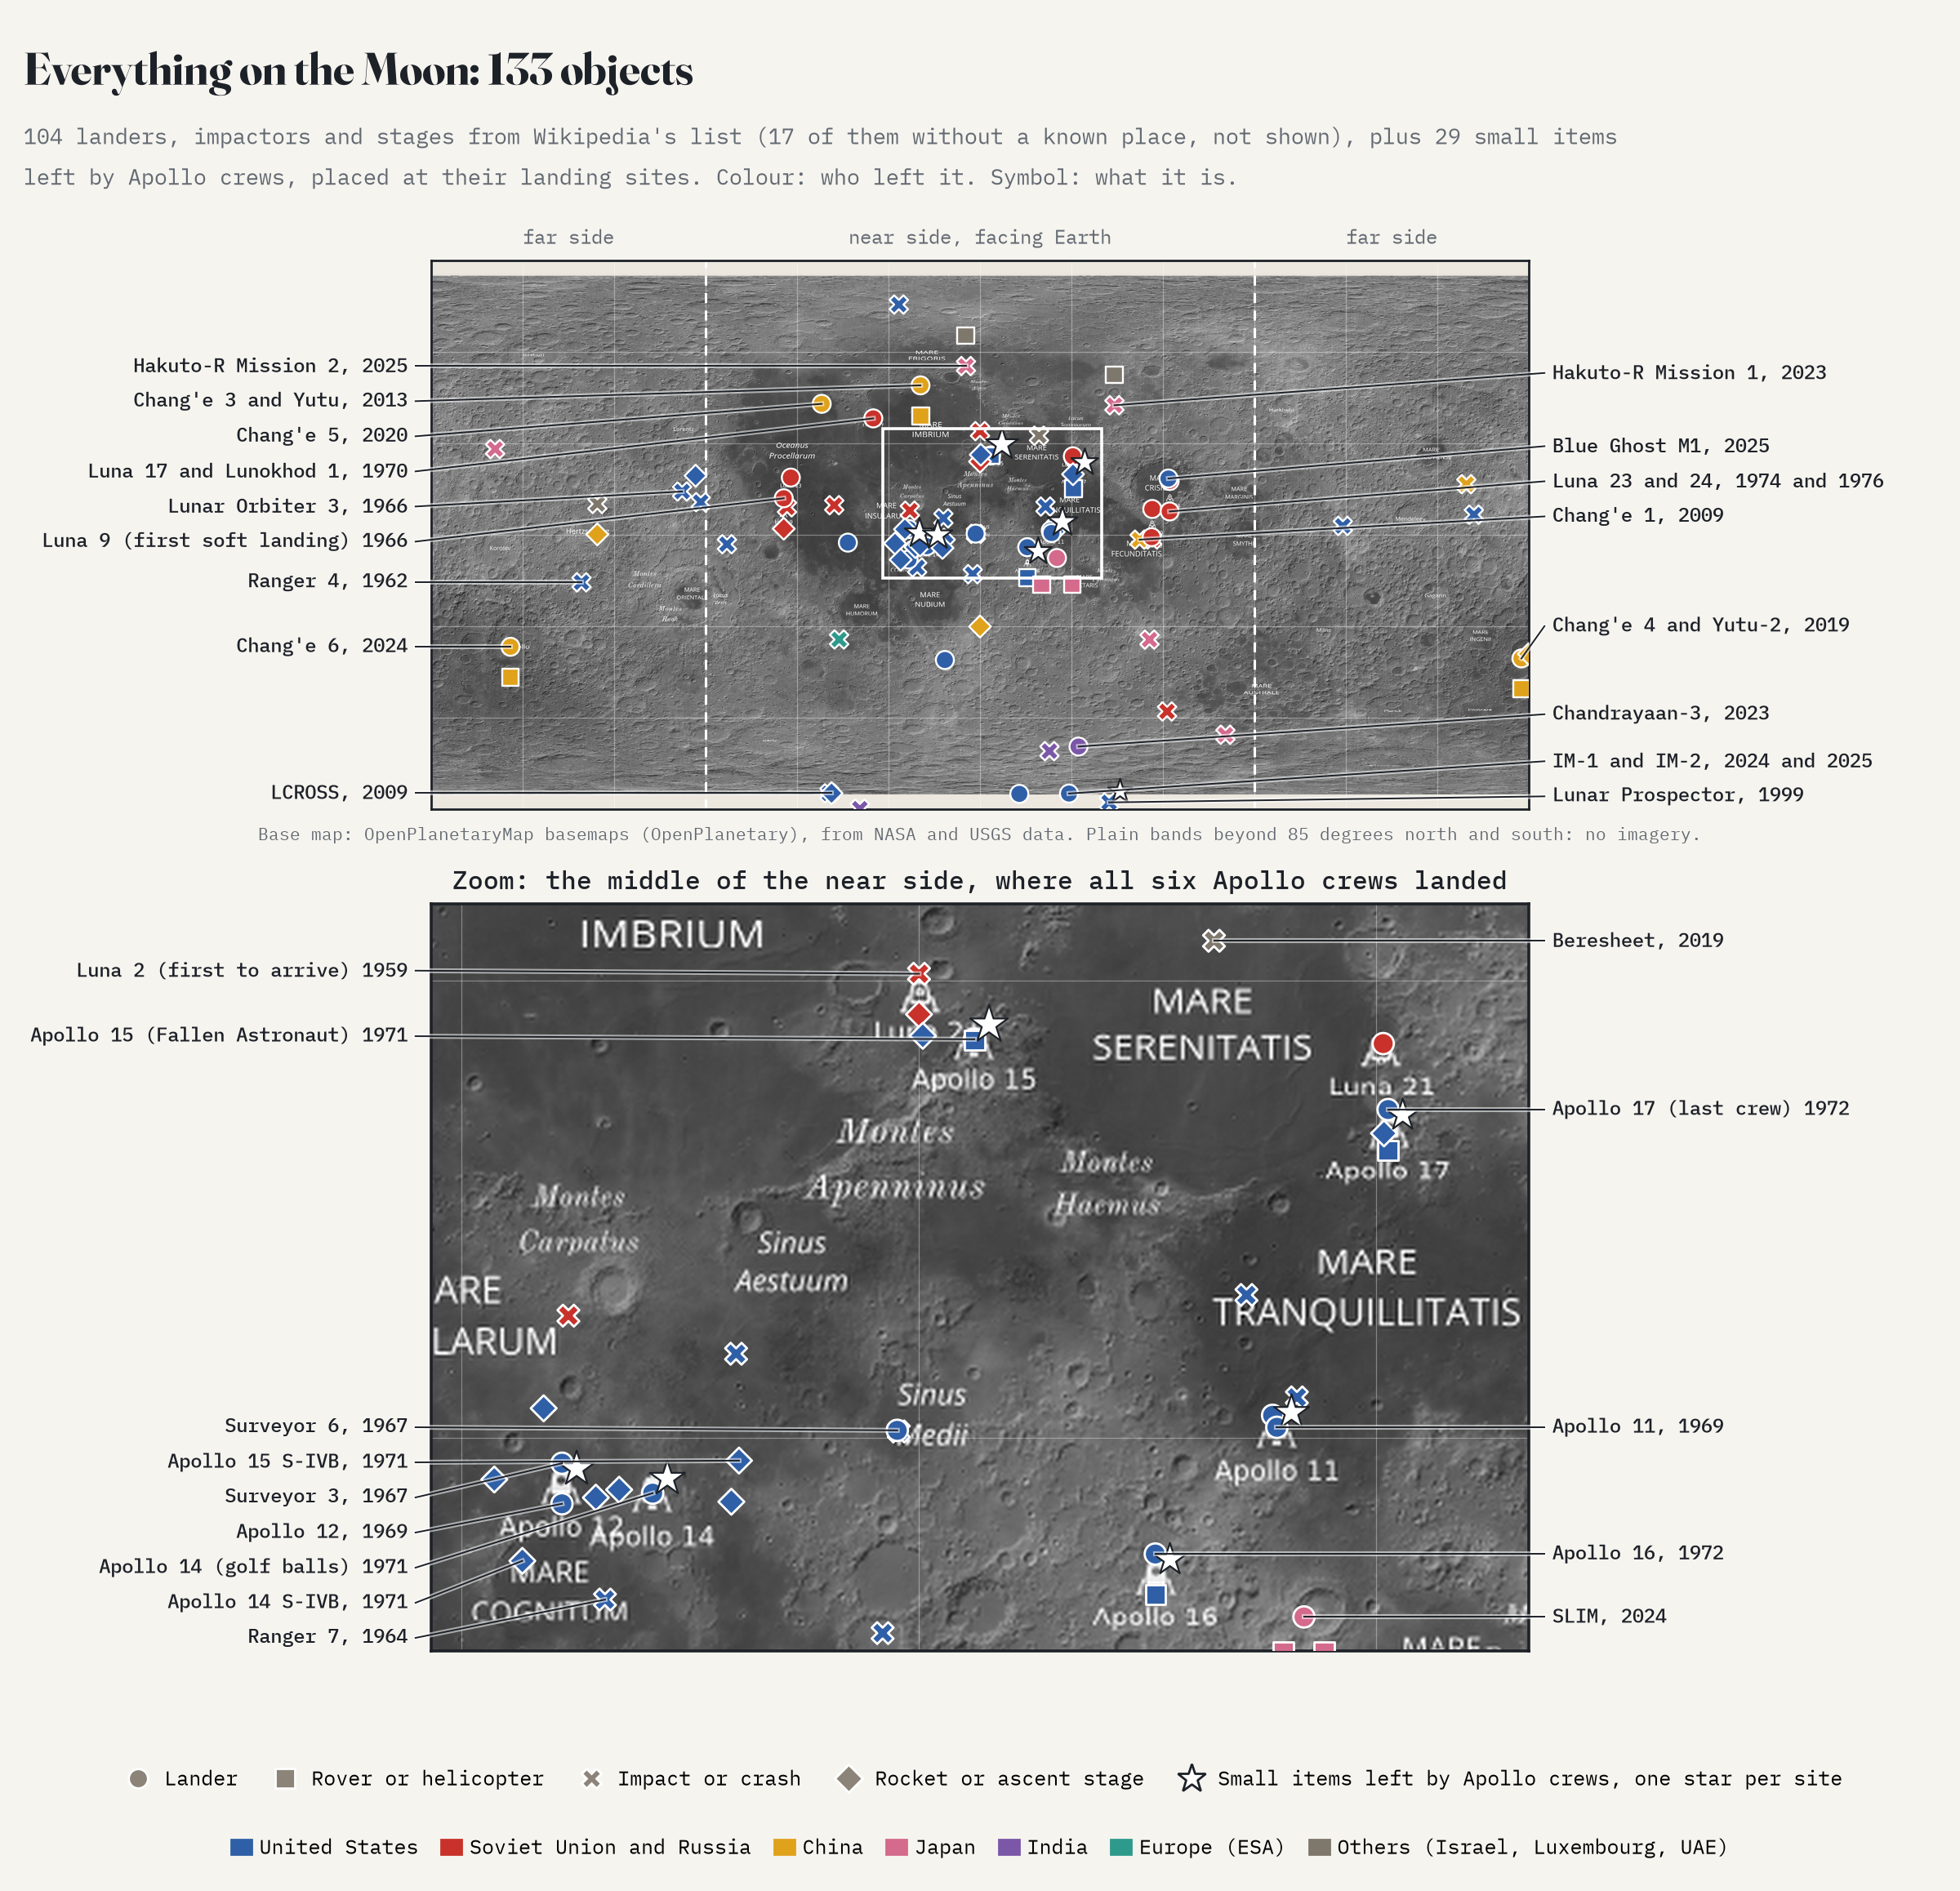
\includegraphics[width=\textwidth]{f_moon_map.png}
\caption{Every located object on the Moon, by type and by who left it, with a zoom on the centre of the near side. Small items are drawn as one star per site. Base map: OpenPlanetaryMap.}\label{fig:moon}\end{figure}

\begin{figure}[tbp]\centering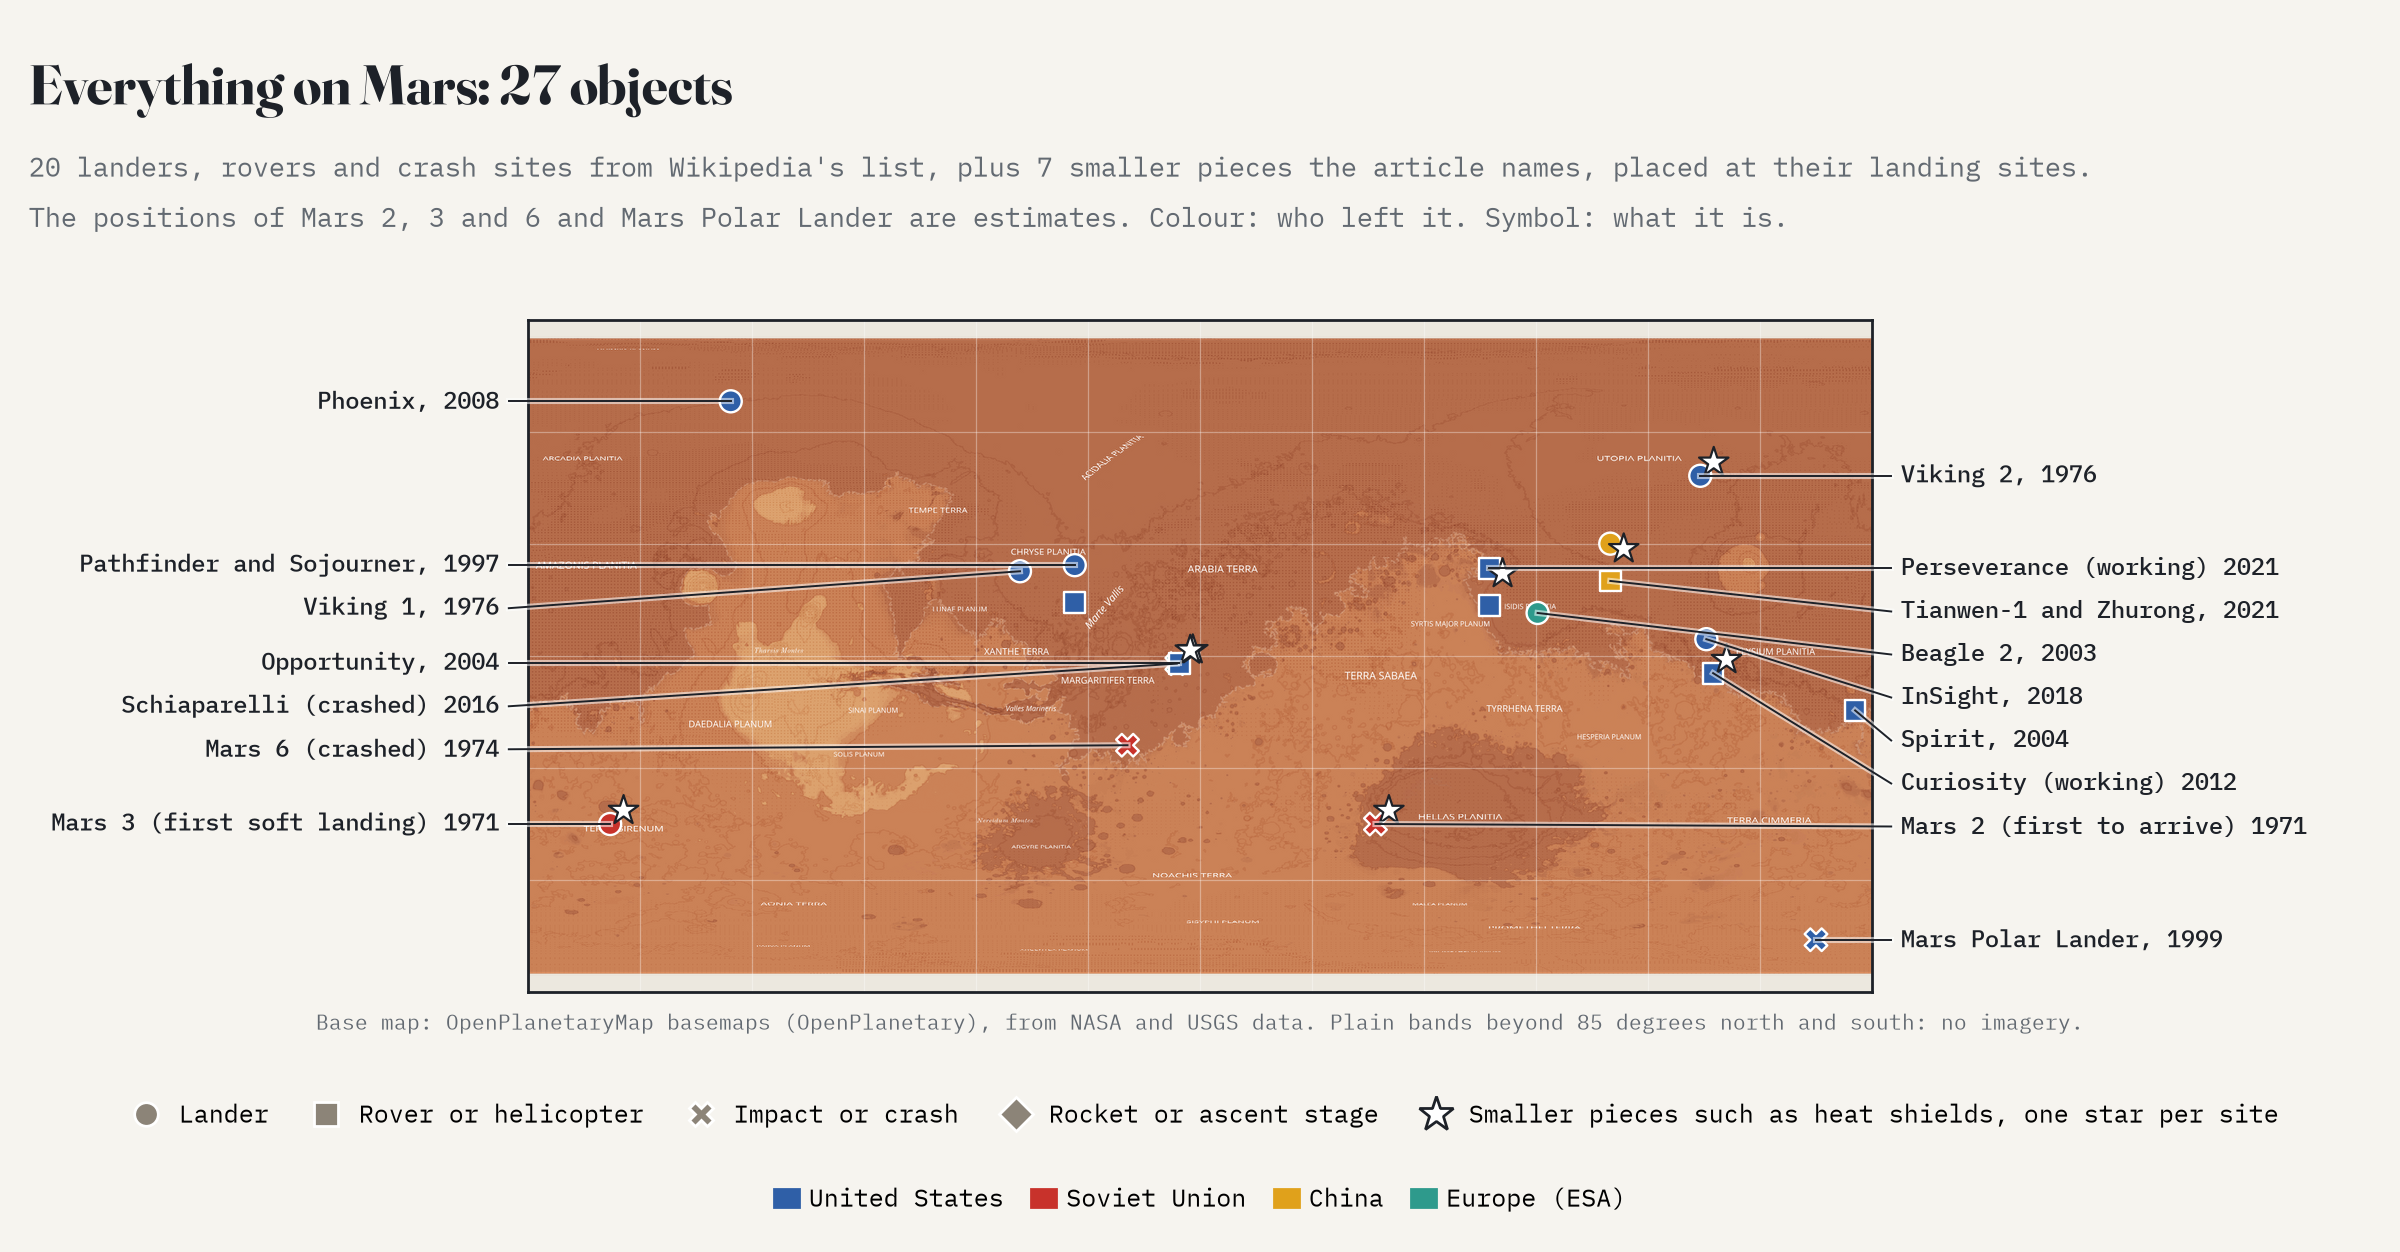
\includegraphics[width=\textwidth]{f_mars_map.png}
\caption{Every object on Mars. The positions of Mars 2, 3 and 6 and Mars Polar Lander are estimates. Base map: OpenPlanetaryMap.}\label{fig:mars}\end{figure}

\begin{figure}[tbp]\centering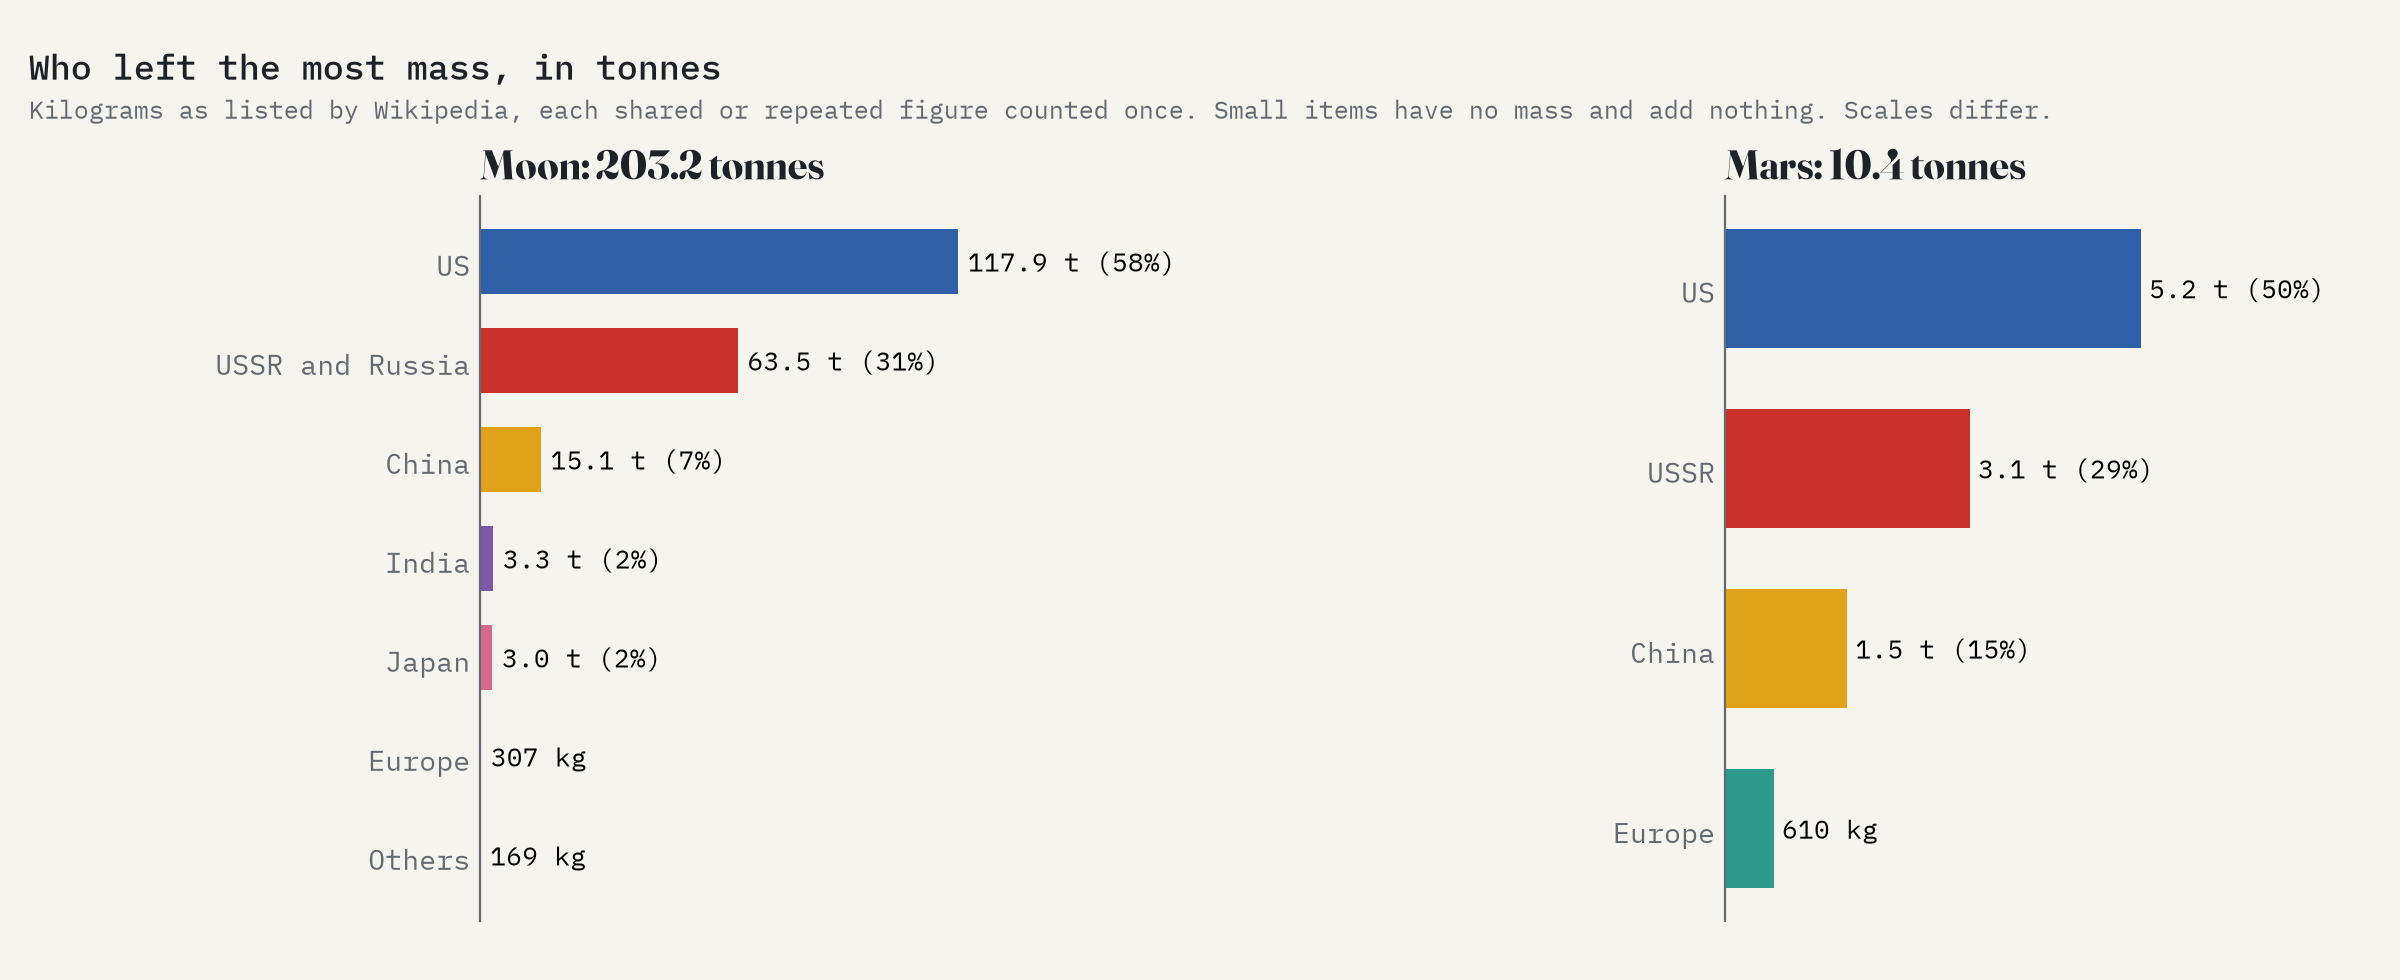
\includegraphics[width=\textwidth]{f_mass.png}
\caption{Mass left on the Moon and Mars by country or agency, each listed figure counted once.}\label{fig:mass}\end{figure}

\begin{table}[tbp]\centering\small\caption{The ten heaviest objects, kilograms as listed.}\label{tab:heavy}\begin{tabular}{llrr}\toprule Object & Body & Year & kg\\\midrule
Apollo 15 S-IVB (S-IVB-510) & Moon & 1971 & 14,036\\
Apollo 14 S-IVB (S-IVB-509) & Moon & 1971 & 14,016\\
Apollo 16 S-IVB (S-IVB-511) & Moon & 1972 & 14,002\\
Apollo 17 S-IVB (S-IVB-512) & Moon & 1972 & 13,960\\
Apollo 13 S-IVB (S-IVB-508) & Moon & 1970 & 13,454\\
Luna 2 rocket third stage (Vostok) & Moon & 1959 & 9,100\\
Luna 24 descent stage & Moon & 1976 & 5,800\\
Luna 20 descent stage & Moon & 1972 & 5,727\\
Luna 17 and Lunokhod 1 & Moon & 1970 & 5,600\\
Luna 23 & Moon & 1974 & 5,600\\
\bottomrule\end{tabular}\end{table}

\begin{figure}[tbp]\centering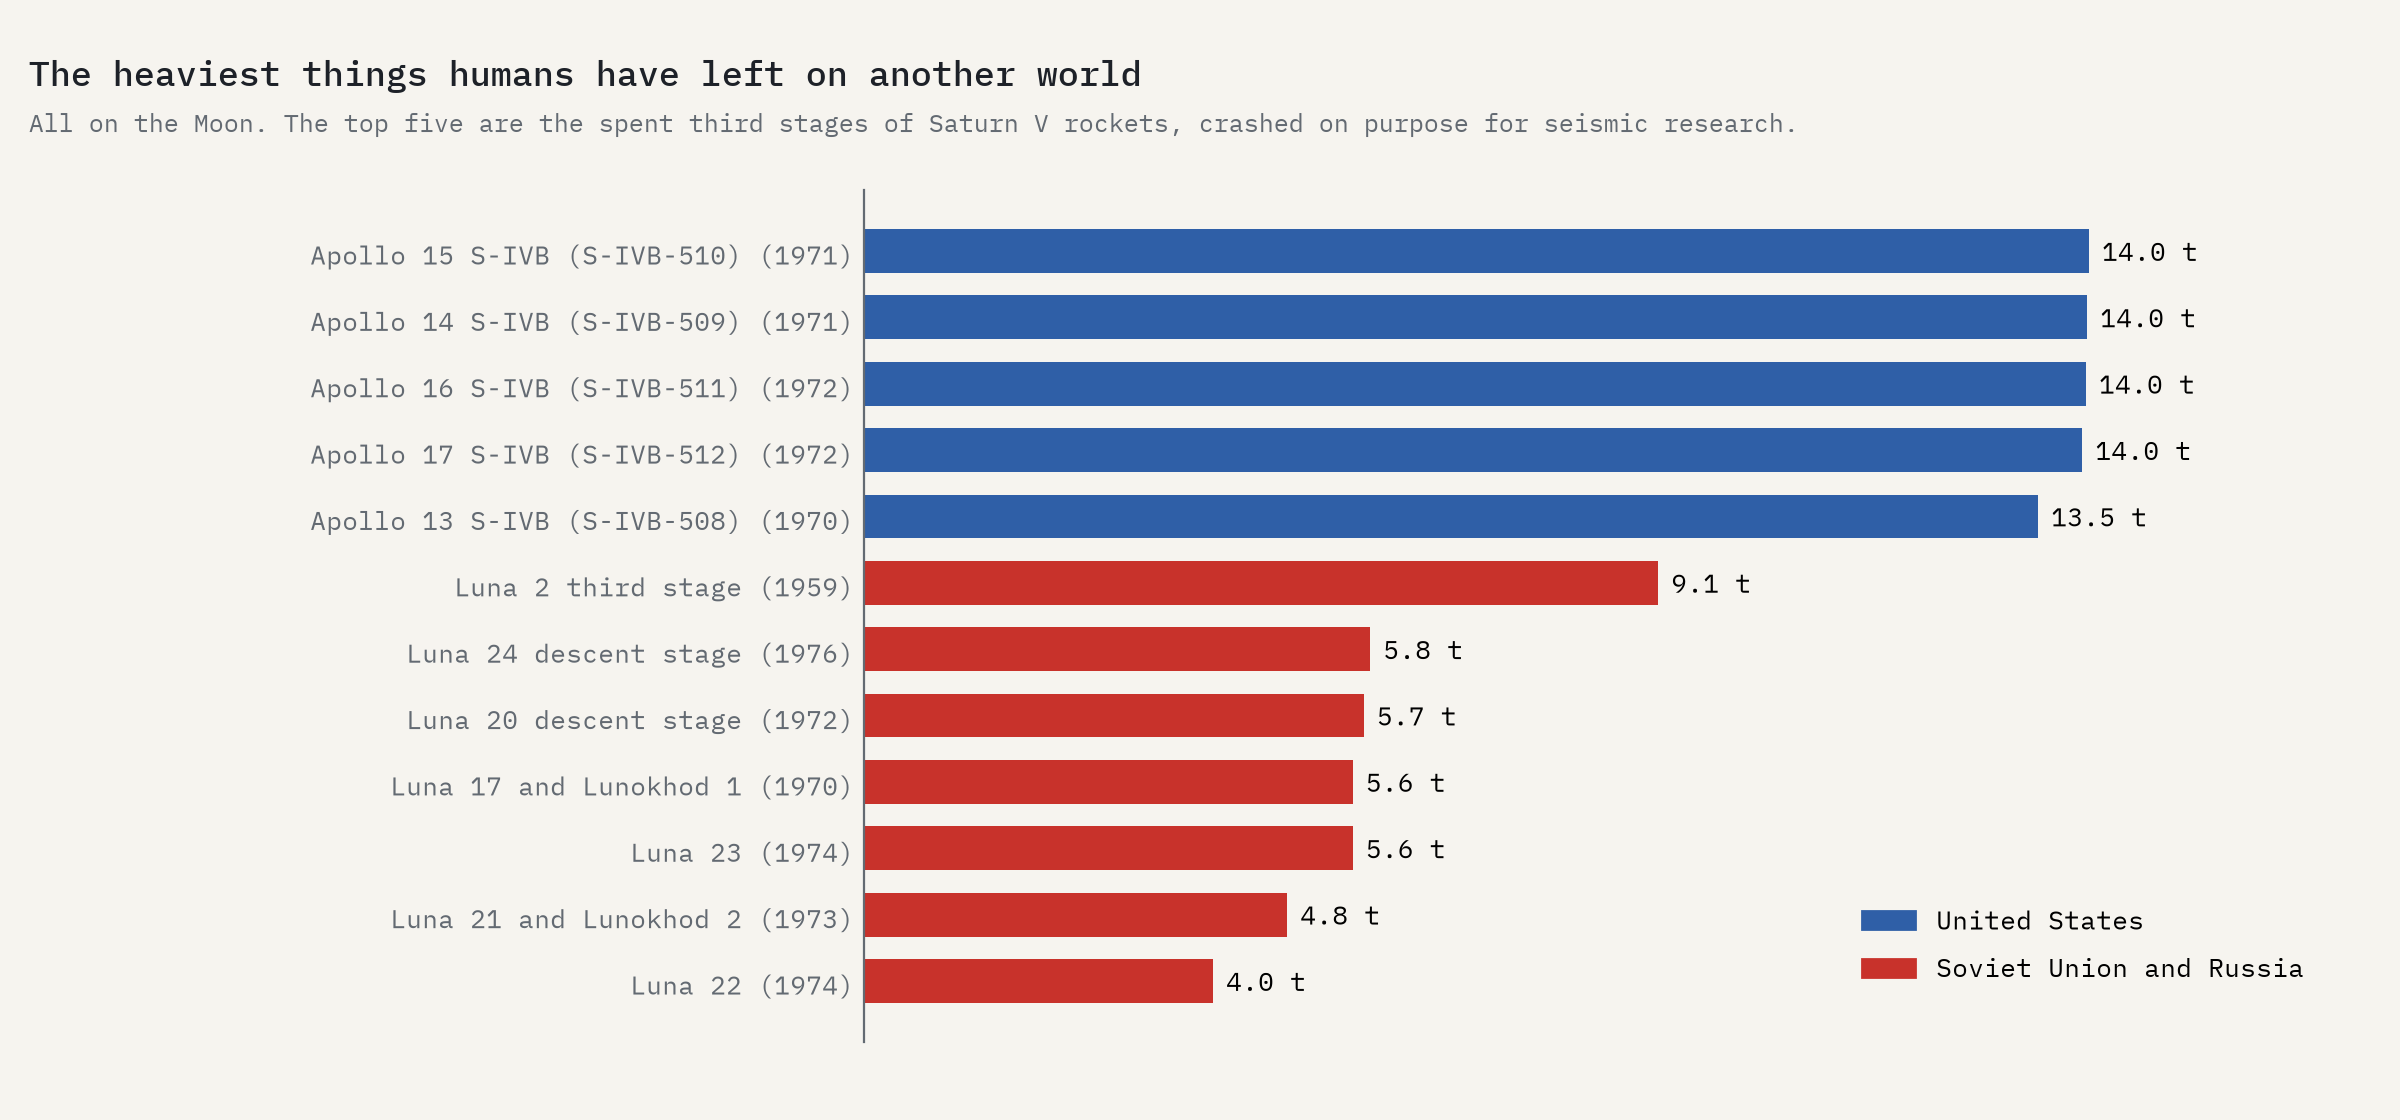
\includegraphics[width=\textwidth]{f_heaviest.png}
\caption{The twelve heaviest objects, all on the Moon.}\label{fig:heavy}\end{figure}

\subsection{When}
Arrivals came in two waves (Figure~\ref{fig:decades}). The first object, Luna 2, struck the Moon on 13 September 1959; 34 table objects arrived in the 1960s and 28 in the 1970s. After Luna 24 in 1976 no listed object reached the Moon until 1990. The 2000s brought 7 and the 2010s 9, mostly hard impacts; the 2020s have already brought 20. Of these 9 objects in the table were built or flown by companies (SpaceIL, LuxSpace, ispace and ispace Europe, Intuitive Machines, Firefly Aerospace and SpaceX), and 3 of them landed softly. The first object on Mars arrived on 27 November 1971 (Mars 2); Mars received 5 table objects in the 1970s and 5 so far in the 2020s.

\begin{figure}[tbp]\centering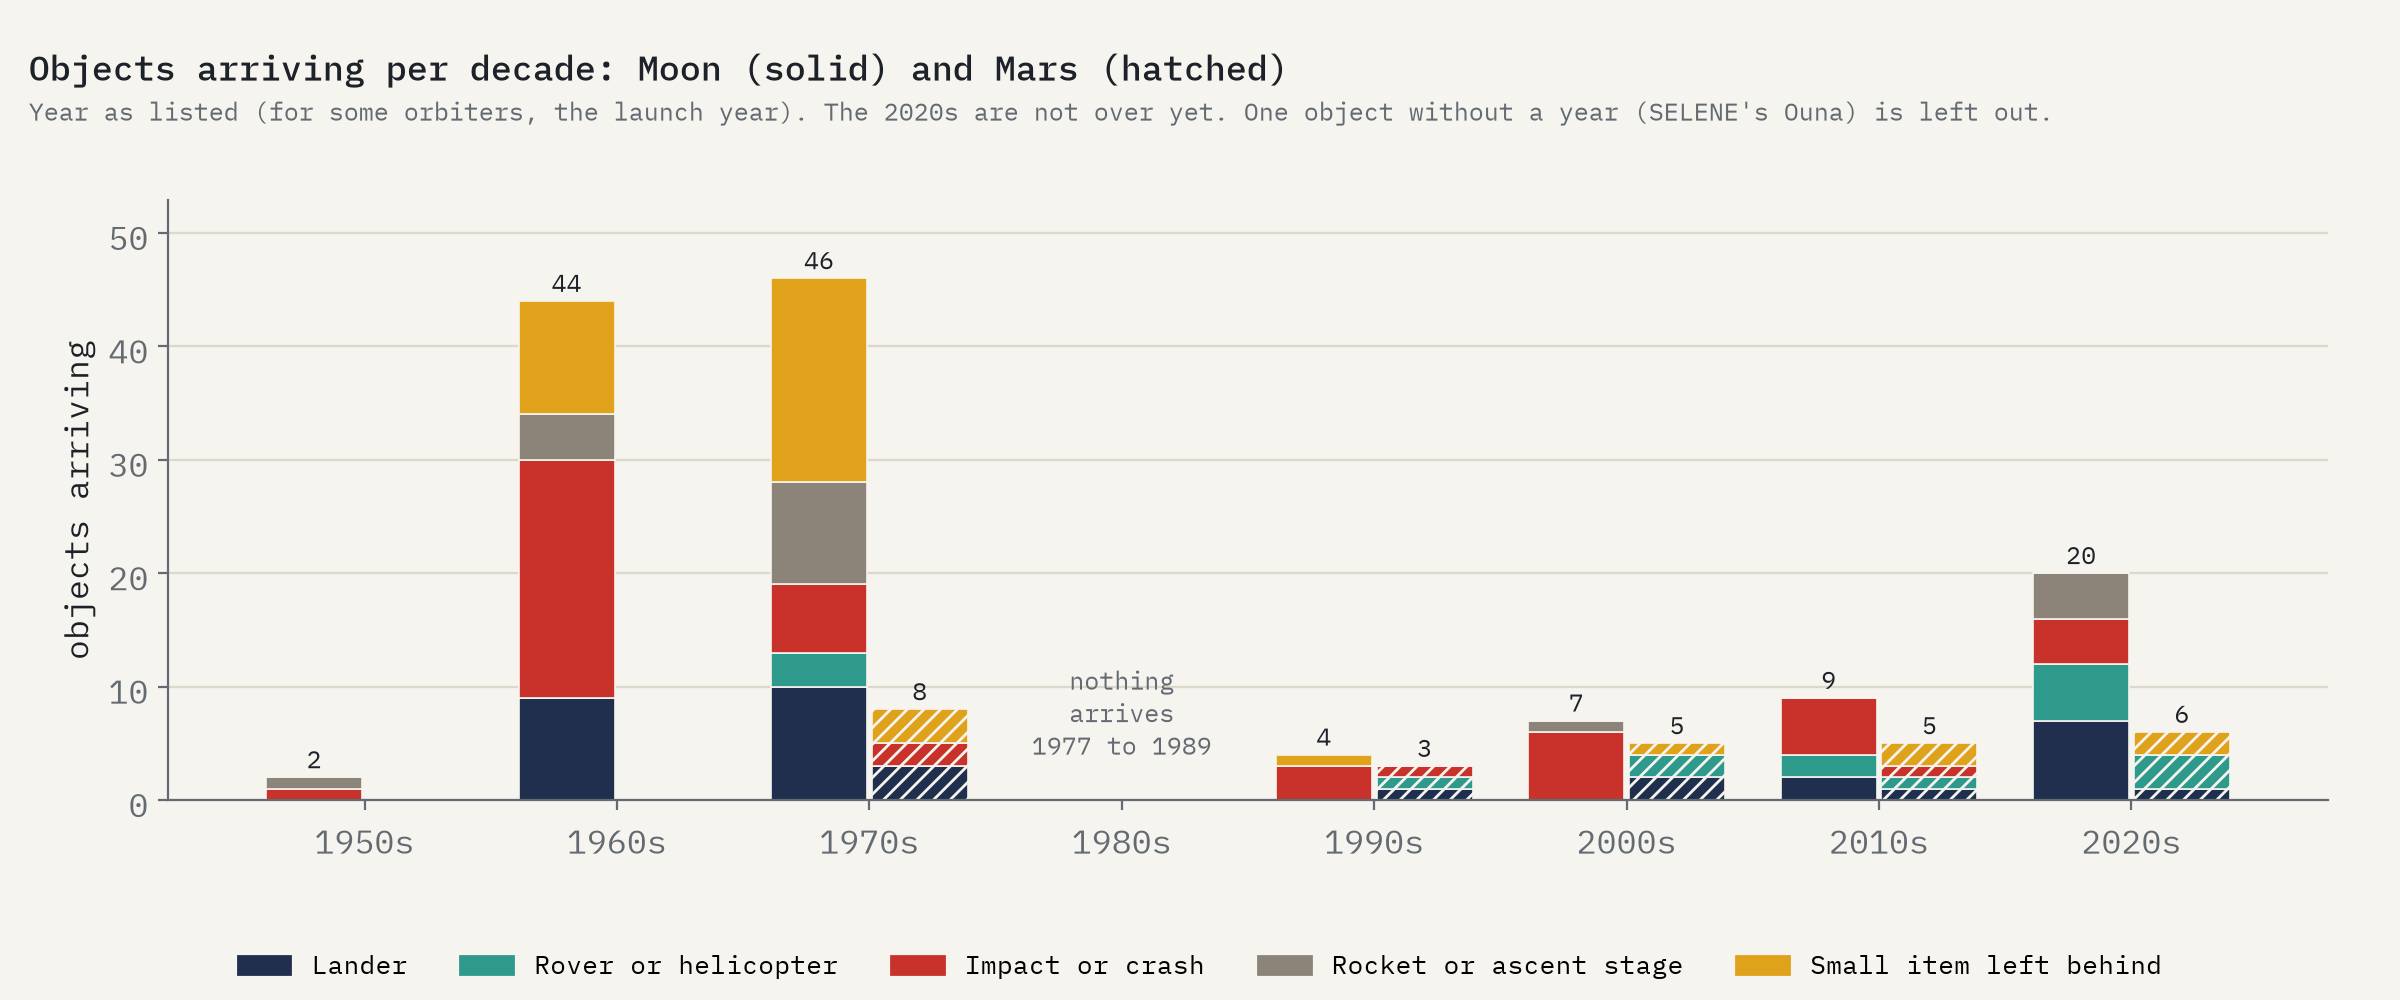
\includegraphics[width=\textwidth]{f_decades.png}
\caption{Objects arriving on the Moon and Mars per decade, by type. Years as listed in the tables.}\label{fig:decades}\end{figure}

\subsection{Crashed or landed, and still working}
Of the 104 Moon rows, 36 (35\%) arrived softly and 68 hard; the article's own summary row speaks of ``40 major objects landed softly'', a broader count that the row colours do not reproduce. Of the 20 Mars rows, 16 arrived softly (Figure~\ref{fig:status}). Only three lunar objects are coloured operational, all Chinese (the Chang'e 3 and Chang'e 4 landers and the Yutu-2 rover); the article's introduction also names SLIM as still in use. On Mars, Curiosity and Perseverance are operating. The Moon list adds that the retroreflectors left by Apollo 11, 14 and 15 and carried by Lunokhod 1, Lunokhod 2 and Chandrayaan-3 are still used for laser ranging, and the ALSEP article that they are the only Apollo experiments still in use; the five ALSEP stations were supported until 30 September 1977.

\begin{figure}[tbp]\centering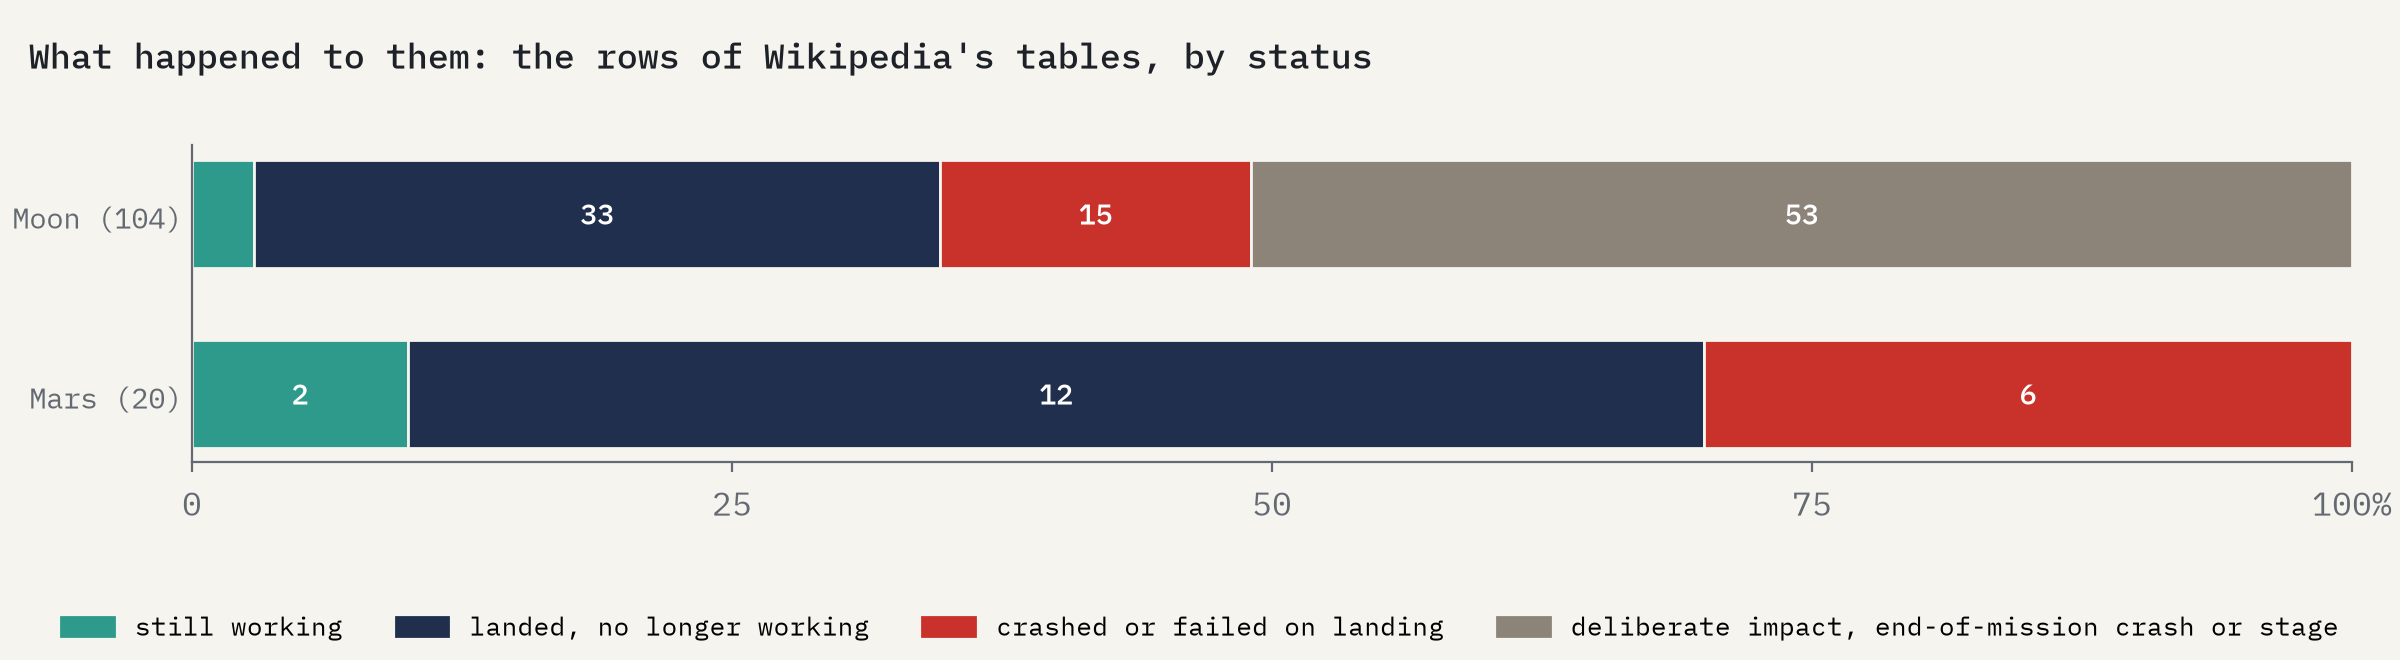
\includegraphics[width=\textwidth]{f_status.png}
\caption{Status of every row of the two tables, from the row colours.}\label{fig:status}\end{figure}

\subsection{Landing success}
The landings list records 40 soft landing attempts on the Moon, of which 28 (70.0\%) succeeded, and 16 on Mars, of which 11 (68.8\%) succeeded (Table~\ref{tab:land}, Figure~\ref{fig:landing}). The first successful lunar soft landing was Luna 9, 3 February 1966. China succeeded in all 4 of its lunar attempts and in its single Mars attempt; the Soviet Union and Russia in 8 of 14 on the Moon and 1 of 3 on Mars. Since 2019, 8 of 13 lunar attempts have succeeded, and 3 of the 6 commercial ones.

\begin{table}[tbp]\centering\small\caption{Soft landing attempts and successes by country (List of landings on extraterrestrial bodies).}\label{tab:land}\begin{tabular}{llrrrr}\toprule Body & Who & Attempts & Succeeded & Rate & First attempt\\\midrule
Moon & United States & 16 & 14 & 88\% & 1966\\
Moon & Soviet Union and Russia & 14 & 8 & 57\% & 1965\\
Moon & China & 4 & 4 & 100\% & 2013\\
Moon & Japan & 3 & 1 & 33\% & 2023\\
Moon & India & 2 & 1 & 50\% & 2019\\
Moon & Israel & 1 & 0 & 0\% & 2019\\
\midrule Moon & All & 40 & 28 & 70\% & \\
\midrule
Mars & United States & 10 & 9 & 90\% & 1976\\
Mars & Soviet Union & 3 & 1 & 33\% & 1971\\
Mars & Europe (ESA) & 2 & 0 & 0\% & 2003\\
Mars & China & 1 & 1 & 100\% & 2021\\
\midrule Mars & All & 16 & 11 & 69\% & \\
\bottomrule\end{tabular}\end{table}

\begin{figure}[tbp]\centering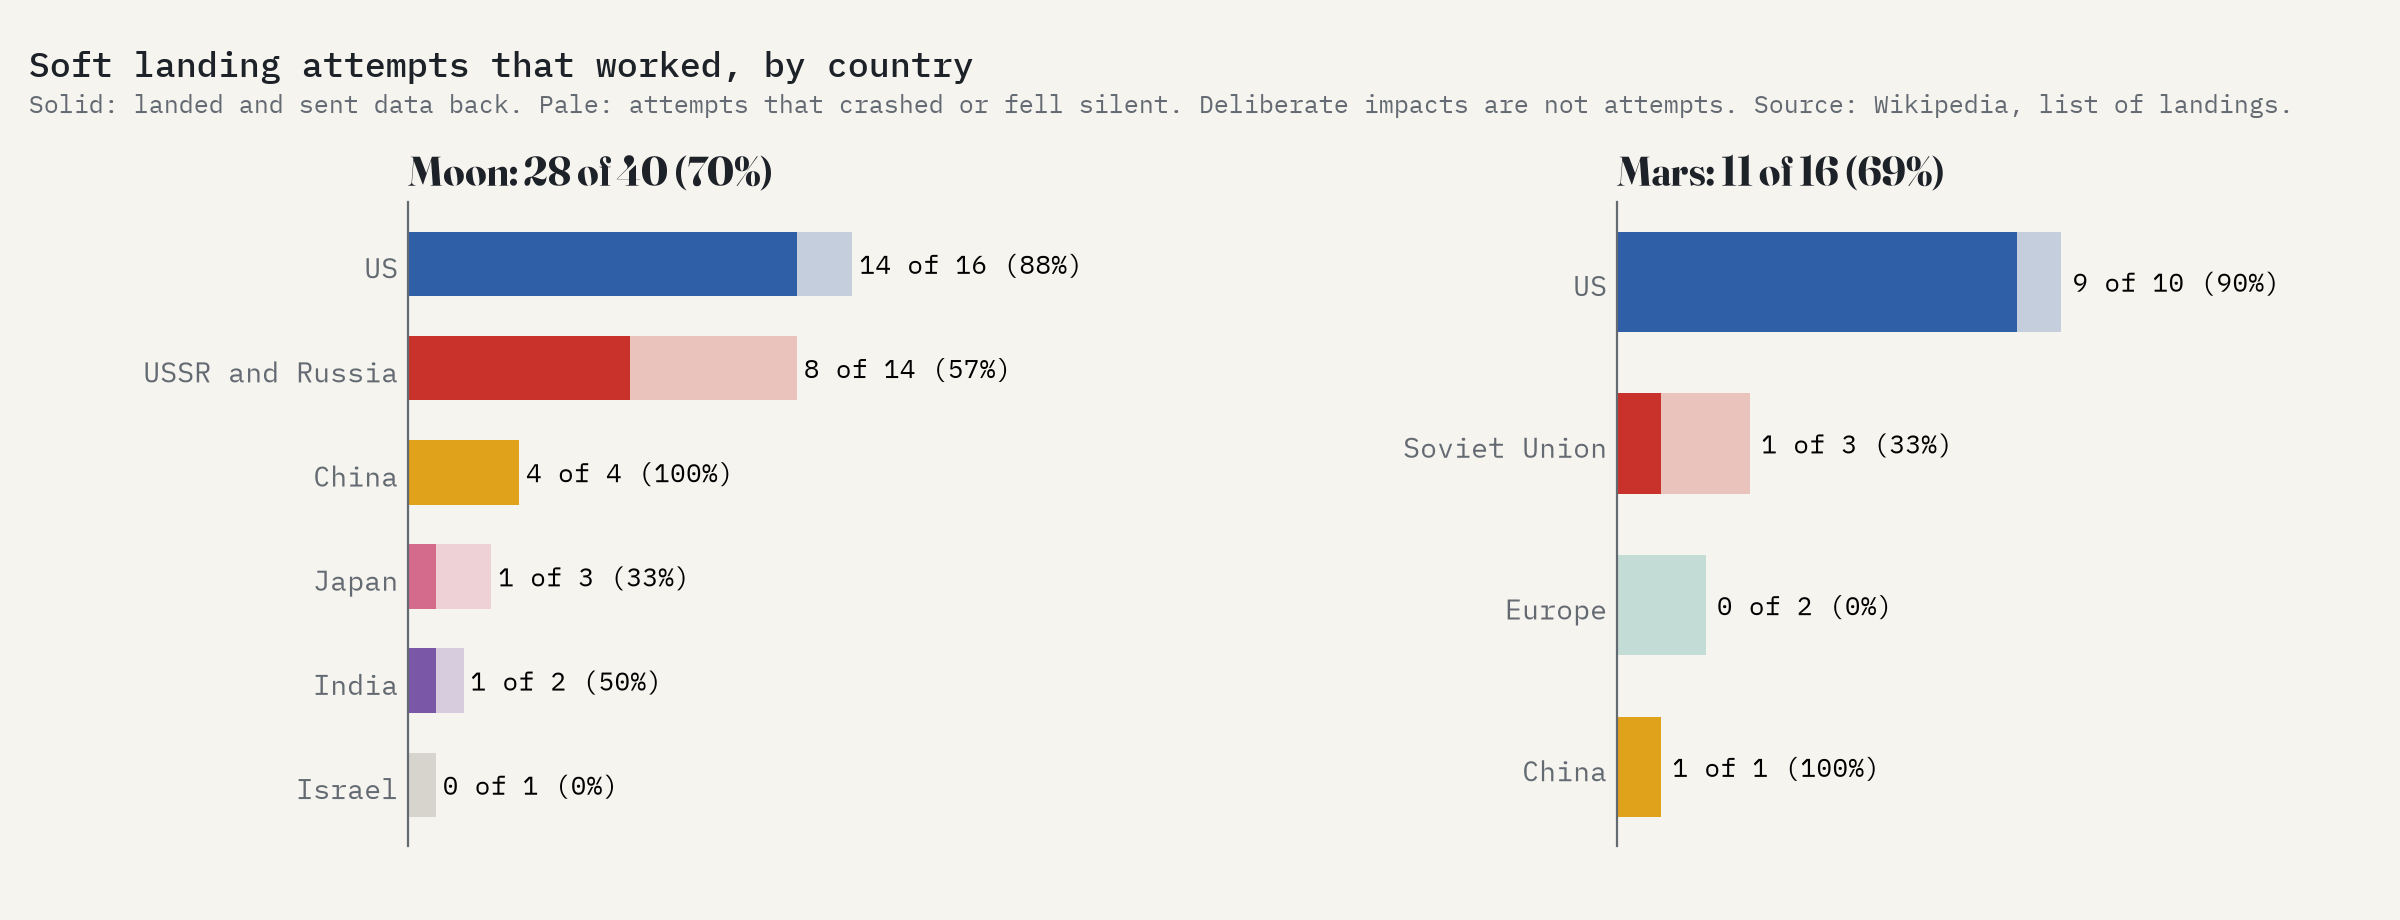
\includegraphics[width=\textwidth]{f_landing.png}
\caption{Soft landing attempts and successes by country.}\label{fig:landing}\end{figure}

\subsection{Near side and far side}
Of the 87 lunar table objects with a position, 15 (17.2\%) lie on the far side, although it is half of the surface. Most of them hit the surface hard; the only soft arrivals there are China's Chang'e 4 lander and Yutu-2 rover and the Chang'e 6 lander and its Jinchan rover.

\subsection{Small items}
The 29 small lunar items (Table~\ref{tab:items}) include the six American flags, of which ``five of the six \ldots{} are still standing'' according to LROC images \citep{wikimoonlanding}; the six ladder plaques; the Apollo 11 goodwill messages disc; Alan Bean's silver astronaut pin; Alan Shepard's golf balls; David Scott's Bible; the 8.9 cm Fallen Astronaut and its plaque naming 8 American astronauts and 6 Soviet cosmonauts \citep{wikifallen}; three laser ranging retroreflectors; the EASEP and five ALSEP packages \citep{wikialsep}; a discarded fuel transfer tool; and Eugene Shoemaker's ashes, carried by Lunar Prospector. Some objects often mentioned, such as the falcon feather from Apollo 15 or Charles Duke's family photograph, are not named in these sources and are not included.

\begin{footnotesize}\begin{longtable}{p{8.2cm}lp{3.4cm}r}\caption{Small items added from the articles' text, placed at their landing sites.}\label{tab:items}\\\toprule Item & Body & Mission & Year\\\midrule\endhead
Apollo 11 United States flag & Moon & Apollo 11 & 1969\\
Apollo 12 United States flag & Moon & Apollo 12 & 1969\\
Apollo 14 United States flag & Moon & Apollo 14 & 1971\\
Apollo 15 United States flag & Moon & Apollo 15 & 1971\\
Apollo 16 United States flag & Moon & Apollo 16 & 1972\\
Apollo 17 United States flag & Moon & Apollo 17 & 1972\\
Apollo 11 commemorative plaque on the Lunar Module ladder & Moon & Apollo 11 & 1969\\
Apollo 12 commemorative plaque on the Lunar Module ladder & Moon & Apollo 12 & 1969\\
Apollo 14 commemorative plaque on the Lunar Module ladder & Moon & Apollo 14 & 1971\\
Apollo 15 commemorative plaque on the Lunar Module ladder & Moon & Apollo 15 & 1971\\
Apollo 16 commemorative plaque on the Lunar Module ladder & Moon & Apollo 16 & 1972\\
Apollo 17 commemorative plaque on the Lunar Module ladder & Moon & Apollo 17 & 1972\\
Apollo 11 goodwill messages disc & Moon & Apollo 11 & 1969\\
Silver astronaut pin left by Alan Bean for Clifton C. Williams & Moon & Apollo 12 & 1969\\
Golf balls hit by Alan Shepard & Moon & Apollo 14 & 1971\\
Bible left by David Scott & Moon & Apollo 15 & 1971\\
Fallen Astronaut statuette & Moon & Apollo 15 & 1971\\
Fallen Astronaut memorial plaque (14 names) & Moon & Apollo 15 & 1971\\
Apollo 11 Laser Ranging Retroreflector & Moon & Apollo 11 & 1969\\
Apollo 14 Laser Ranging Retroreflector & Moon & Apollo 14 & 1971\\
Apollo 15 Laser Ranging Retroreflector & Moon & Apollo 15 & 1971\\
Apollo 11 Early Apollo Scientific Experiments Package (EASEP) & Moon & Apollo 11 & 1969\\
Apollo 12 Apollo Lunar Surface Experiments Package (ALSEP) & Moon & Apollo 12 & 1969\\
Apollo 14 Apollo Lunar Surface Experiments Package (ALSEP) & Moon & Apollo 14 & 1971\\
Apollo 15 Apollo Lunar Surface Experiments Package (ALSEP) & Moon & Apollo 15 & 1971\\
Apollo 16 Apollo Lunar Surface Experiments Package (ALSEP) & Moon & Apollo 16 & 1972\\
Apollo 17 Apollo Lunar Surface Experiments Package (ALSEP) & Moon & Apollo 17 & 1972\\
Apollo 12 ALSEP fuel transfer tool (discarded) & Moon & Apollo 12 & 1969\\
Ashes of Eugene Shoemaker (on Lunar Prospector) & Moon & Lunar Prospector & 1999\\
Soviet pennant on the Mars 2 lander & Mars & Mars 2 & 1971\\
Soviet pennant on the Mars 3 lander & Mars & Mars 3 & 1971\\
Viking 2 surface sampler shroud & Mars & Viking 2 & 1976\\
Opportunity heat shield & Mars & MER-B & 2004\\
Curiosity (MSL) counterweights ejected during descent & Mars & Mars Science Laboratory & 2012\\
Schiaparelli heat shields and parachute & Mars & ExoMars 2016 & 2016\\
Three Forks Sample Depot (Perseverance sample tubes) & Mars & Mars 2020 & 2022\\
\bottomrule\end{longtable}\end{footnotesize}

\subsection{Where the sources disagree}
For 86 objects both the object tables and the landings list give coordinates. They differ by more than one degree of arc for 8 (Table~\ref{tab:disagree}), among them Luna 5, Surveyor 2, IM-1 and IM-2, Mars 2 and Mars Polar Lander. Some differences reflect uncertain crash sites; the Mars Polar Lander positions are in different hemispheres. I keep the object tables' positions throughout and publish the alternatives in the data.

\begin{table}[tbp]\centering\small\caption{Objects whose positions in the object tables and in the landings list differ by more than one degree of arc.}\label{tab:disagree}\begin{tabular}{p{6.2cm}llr}\toprule Object & Object table & Landings list & Degrees\\\midrule
Luna 5 & 8.00N 23.00W & 31.00S 8.00W & 41.6\\
Luna 8 & 9.10N 63.30W & 9.60N 62.00W & 1.4\\
Lunar Orbiter 1 & 6.70N 162.00E & 6.35N 160.72E & 1.3\\
Surveyor 2 & 5.50N 12.00W & 4.00S 11.00W & 9.6\\
IM-1 Odysseus lander and EagleCam & 84.90S 12.90E & 80.13S 1.44E & 5.0\\
IM-2 Athena lander, with MAPP LV1, Micro-Nova, AstroAnt and Yaoki & 84.79S 29.20E & 85.00S 31.00W & 5.1\\
Mars 2 lander and PrOP-M rover & 45.00S 47.00E & 45.00S 30.00W & 52.2\\
Mars Polar Lander and Deep Space 2 probes & 76.00S 165.00E & 73.00N 150.00E & 149.3\\
\bottomrule\end{tabular}\end{table}

\section{Limitations}
First, Wikipedia is an edited compilation, not a primary record, and it changes: the inventory describes the revisions cited. Second, the tables are partial by their own account; the Mars list omits springs, fragments, parachutes and heat shields, and many small Apollo items (tools, bags, equipment) are not named anywhere in these sources. Third, masses mix dry and launch masses and include bounds, so totals are approximate. Fourth, the type classification is mine and some rows hold several objects. Fifth, small items are placed at their landing sites. Sixth, web maps cannot show latitudes beyond about 85 degrees, so the interactive map draws polar objects at its edge; the static figures and the page's polar chart show them properly. Seventh, landing success counts only attempts that reached their target.

\section{Conclusion}
About 0 tonnes of hardware lie on the Moon and about 0 on Mars. Most of the lunar mass is the legacy of a few years of the Cold War race, and a third of it is five rocket stages. Almost all of it is dead. The 2020s are adding objects faster than any decade since the 1970s, from more countries and from companies, with mixed results: landing on the Moon is still far from routine, and Mars remains harder. A consistent, open inventory makes those patterns visible, and shows how much of this archive is still described only loosely.

\section*{Data and code availability}
The interactive map is at \url{https://maps.tristanhotham.com/moon-mars/}. Data and code are at \url{https://github.com/Tristan-Hotham/moon-mars} and archived with this paper at https://doi.org/10.5281/zenodo.23872995. The object table derived from Wikipedia is released under CC BY-SA 4.0; other derived data and text under CC BY 4.0; code under the MIT licence.

\section*{AI statement}
I wrote the text, with drafting and editing assistance from Claude (Anthropic), which also helped prepare the analysis code. I reviewed and checked all text and results.

\begin{thebibliography}{12}
\bibitem[OpenPlanetary(2026)]{opm} OpenPlanetary (2026) OpenPlanetaryMap basemaps: opm-moon-basemap-v0-1 and opm-mars-basemap-v0-2, from NASA and USGS data.
\bibitem[Wikipedia(2026a)]{wikimoon} Wikipedia contributors (2026) List of artificial objects on the Moon (revision 1370338372). CC BY-SA 4.0. \url{https://en.wikipedia.org/wiki/List_of_artificial_objects_on_the_Moon}
\bibitem[Wikipedia(2026b)]{wikimars} Wikipedia contributors (2026) List of artificial objects on Mars (revision 1373656289). CC BY-SA 4.0. \url{https://en.wikipedia.org/wiki/List_of_artificial_objects_on_Mars}
\bibitem[Wikipedia(2026c)]{wikilandings} Wikipedia contributors (2026) List of landings on extraterrestrial bodies (revision 1372275847). CC BY-SA 4.0. \url{https://en.wikipedia.org/wiki/List_of_landings_on_extraterrestrial_bodies}
\bibitem[Wikipedia(2026d)]{wikimoonlanding} Wikipedia contributors (2026) Moon landing (revision 1380159374). CC BY-SA 4.0. \url{https://en.wikipedia.org/wiki/Moon_landing}
\bibitem[Wikipedia(2026e)]{wikifallen} Wikipedia contributors (2026) Fallen Astronaut (revision 1359569457). CC BY-SA 4.0. \url{https://en.wikipedia.org/wiki/Fallen_Astronaut}
\bibitem[Wikipedia(2026f)]{wikialsep} Wikipedia contributors (2026) Apollo Lunar Surface Experiments Package (revision 1354555151). CC BY-SA 4.0. \url{https://en.wikipedia.org/wiki/Apollo_Lunar_Surface_Experiments_Package}
\bibitem[Wikipedia(2026g)]{wikilrv} Wikipedia contributors (2026) Lunar Roving Vehicle (revision 1380980067). CC BY-SA 4.0. \url{https://en.wikipedia.org/wiki/Lunar_Roving_Vehicle}
\bibitem[Wikipedia(2026h)]{wikimissionsmoon} Wikipedia contributors (2026) List of missions to the Moon (revision 1380188613). CC BY-SA 4.0. \url{https://en.wikipedia.org/wiki/List_of_missions_to_the_Moon}
\bibitem[Wikipedia(2026i)]{wikimissionsmars} Wikipedia contributors (2026) List of missions to Mars (revision 1383270651). CC BY-SA 4.0. \url{https://en.wikipedia.org/wiki/List_of_missions_to_Mars}
\end{thebibliography}
\end{document}
